\documentclass[11pt]{article}

% packages
\usepackage{enumerate}
\usepackage{fancyhdr}
\usepackage{extramarks}
\usepackage{amsmath}
\usepackage{amsthm}
\usepackage{amssymb}
%\usepackage{amsfonts}
\usepackage{tikz}
\usepackage[plain]{algorithm}
\usepackage{algpseudocode}
\usepackage{lastpage}
\usepackage{units}
\usepackage[margin=0.75in]{geometry}
\usepackage{pgfplots}
\pgfplotsset{compat=1.16}
\usepackage{sectsty}
\usepackage{hyperref}
\usepackage{multicol}
\usepackage{mathtools}
\usepackage{tikz}
\usetikzlibrary{matrix}
\usepackage{listings}
\usepackage[plain]{algorithm}
\usepackage{algpseudocode}

\definecolor{sblue}{HTML}{5292c0}
\definecolor{sgreen}{HTML}{93c47d}
\definecolor{sorange}{HTML}{e69138}
\definecolor{codeblue}{rgb}{0.29296875, 0.51953125, 0.68359375}
\definecolor{codegreen}{rgb}{0.47265625, 0.62890625, 0.40234375}
\definecolor{codegray}{rgb}{0.95703125, 0.95703125, 0.95703125}
\definecolor{codecrimson}{rgb}{0.87109375,0.3984375,0.3984375}

\lstset{frame=tb,
  backgroundcolor=\color{codegray},
  aboveskip=3mm,
  belowskip=3mm,
  showstringspaces=false,
  columns=flexible,
  basicstyle={\small\ttfamily},
  numbers=left,
  numberstyle=\tiny\color{gray},
  keywordstyle=\color{codeblue},
  commentstyle=\color{codegreen},
  stringstyle=\color{codecrimson},
  breaklines=true,
  breakatwhitespace=true,
  tabsize=4,
  frame=tlbr,framesep=4pt,framerule=0pt,
  literate={`}{\`}1,
}

% colors
\definecolor{sblue}{HTML}{5292c0}
\definecolor{sgreen}{HTML}{93c47d}
\definecolor{sorange}{HTML}{e69138}

% sectioning magic
\counterwithin*{equation}{section}
%\numberwithin{equation}{section}

% fonts
\usepackage{fontspec}
\newfontfamily\headerfontlt{ITC Franklin Gothic Std Book}
\newfontfamily\headerfont{ITC Franklin Gothic Std Demi}
\usepackage[urw-garamond]{mathdesign}
\usepackage{garamondx}
\usepackage[italic]{mathastext}

\newcommand{\printsection}[1]{\normalfont\headerfontlt{{{#1}}}}
\newcommand{\printsubsection}[1]{\normalfont\headerfontlt\textcolor{darkgray}{{#1}}}
\newcommand{\printsubsubsection}[1]{\normalfont\headerfontlt{{#1}}}
\allsectionsfont{\printsection}
\subsectionfont{\printsection}
\subsectionfont{\printsubsection}
\subsubsectionfont{\printsubsubsection}


\renewcommand{\headrulewidth}{0.1pt}
\renewcommand{\headrule}{\hbox to\headwidth{\color{gray}\leaders\hrule height \headrulewidth\hfill}}
\renewcommand{\footrulewidth}{0.0pt}

\newcommand{\op}[1]{\textrm{\small\printsubsection{\MakeUppercase{#1}}}\,}
\newcommand{\opns}[1]{\textrm{\small\printsubsection{\MakeUppercase{#1}}}}
\newcommand{\Partial}[1]{\partial\hspace{-0.2ex}{#1}}
\newcommand{\D}[1]{\mathrm{d}#1}
\newcommand{\E}[1]{\mathbb{E}{\left[\,#1\,\right]}}
\newcommand{\var}[1]{\mathrm{var}\left( #1 \right)}
\newcommand{\cov}[1]{\mathrm{cov}\left( #1 \right)}
\newcommand{\pr}[1]{\mathrm{Pr}\left( #1 \right)}
\newcommand{\given}{\,|\,}
\renewcommand{\det}{\mathrm{det\,}}
\renewcommand{\det}[1]{\op{det}\left(#1\right)}
\renewcommand{\ker}{\mathrm{Ker\,}}
\newcommand{\trace}[1]{\op{trace}\left(#1\right)}
\newcommand{\nul}[1]{\op{nul}\left(#1\right)}
\newcommand{\col}[1]{\op{col}\left(#1\right)}
\newcommand{\row}[1]{\op{row}\left(#1\right)}
\newcommand{\rank}[1]{\op{rank}\left(#1\right)}
\renewcommand{\dim}[1]{\op{dim}\left(#1\right)}
\newcommand{\im}{\op{Im\,}}
\newcommand{\reals}{\mathbb{R}}
\newcommand{\complex}{\mathbb{C}}
\renewcommand{\vec}[1]{\mathbf{#1}}
\newcommand*{\matr}[1]{\mathbfit{#1}}
\newcommand*{\tran}{^{\mkern-1.5mu\mathsf{T}}}
\newcommand*{\conj}[1]{\overline{#1}}
\newcommand*{\hermconj}{^{\mathsf{H}}}
\newcommand*{\inv}{^{-1}}

\setlength\parindent{0pt}
\pagecolor{gray!1}


% header/footer
\topmargin=-0.65in
\pagestyle{fancy}\fancyhf{} 
\lhead{\headerfontlt{\textcolor{darkgray}{Satej Soman \textcolor{gray}{$\big/$} CAPP30254, Spring 19 \textcolor{gray}{$\big/$}} Homework 1}}
\rhead{\headerfontlt{\textcolor{gray}{$\big[$} \thepage\ \textcolor{gray}{$\big/$} \pageref{LastPage} \textcolor{gray}{$\big]$}}}

\begin{document}
\begin{titlepage}
\raggedleft\huge\headerfontlt{
\textcolor{darkgray}{Satej Soman\\
CAPP30254: Machine Learning for Public Policy\\
Spring 2019}}

\vspace{240pt}
\Huge\headerfontlt{\textcolor{darkgray}{HW 1\\DIAGNOSTIC ASSIGNMENT}}

\end{titlepage}
\section{Data Acquisition \& Analysis}
\subsection{Chicago Open Data Portal}
Chicago crime data is available, filtered by year, from the Chicago Data Portal (\url{https://data.cityofchicago.org/browse?category=Public\%20Safety}). We can download this data and load it into a Pandas \texttt{DataFrame}:

\begin{lstlisting}[language=Python,numbers=none]
from pathlib import Path

import pandas as pd
import requests

# download crime data if we don't have it locally
base_url = "https://data.cityofchicago.org/api/views/{}/rows.csv?accessType=DOWNLOAD"
crime_resources = { 
    2017: (Path("./crime_data_2017.csv"), "3i3m-jwuy"),
    2018: (Path("./crime_data_2018.csv"), "d62x-nvdr"),
}

for (year, (path, identifier)) in crime_resources.items():
    if not path.exists():
        url = base_url.format(identifier)
        print("{} data not found locally, downloading from {}".format(year, url))
        response = requests.get(url)
        with path.open("wb") as f:
            f.write(response.content)

crime = pd.concat([
    pd.read_csv(crime_resources[2017][0]), 
    pd.read_csv(crime_resources[2018][0])
])
\end{lstlisting}


\subsection{Summary Statistics for Crime Report Data, 2017-2018}

\begin{table}[H]
\centering \renewcommand{\arraystretch}{1.2}
\begin{tabular}{lrrr}
\multicolumn{1}{l|}{year} &    \opns{2017} &    \opns{2018} &     \opns{AVG} \\\hline
\multicolumn{1}{l|}{number of reported crimes} &  268094 &  266246 &  267170 \\
\\ \\
%\end{tabular}
%\end{table}
%\begin{table}[H]
%\centering \renewcommand{\arraystretch}{1.2}
%\begin{tabular}{l|rrr}
\multicolumn{1}{l|}{year} &       \opns{2017} &  \opns{2018} &  \opns{OVERALL} \\\hline
\multicolumn{1}{l|}{crimes involving an arrest}   &  19.53\% &  19.75\% &  19.64\% \\
\multicolumn{1}{l|}{crimes considered domestic}   &  15.90\% &  16.39\% &  16.14\% 
\end{tabular}
\end{table}


{\centering
\hspace{-1in}% This file was created by matplotlib2tikz v0.7.3.
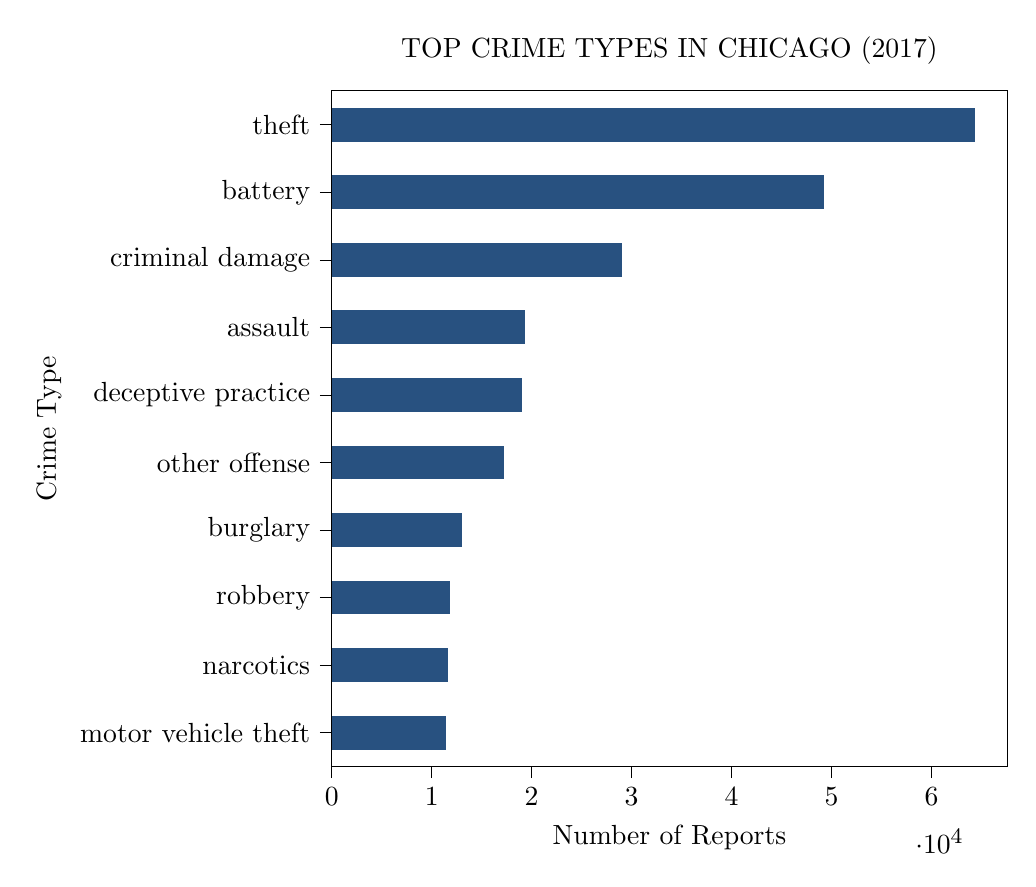
\begin{tikzpicture}

\definecolor{color0}{rgb}{0.156862745098039,0.317647058823529,0.501960784313725}

\begin{axis}[
height=4in,
tick align=outside,
tick pos=left,
title={\printsection{\MakeUppercase{Top Crime Types in Chicago (2017)}}},
width=4in,
x grid style={white!69.01960784313725!black},
xlabel={Number of Reports},
xmin=0, xmax=67562.25,
xtick style={color=black},
y grid style={white!69.01960784313725!black},
ylabel={Crime Type},
ymin=-0.5, ymax=9.5,
ytick style={color=black},
ytick={0,1,2,3,4,5,6,7,8,9},
yticklabels={motor vehicle theft,narcotics,robbery,burglary,other offense,deceptive practice,assault,criminal damage,battery,theft}
]
\draw[fill=color0,draw opacity=0] (axis cs:0,-0.25) rectangle (axis cs:11406,0.25);
\draw[fill=color0,draw opacity=0] (axis cs:0,0.75) rectangle (axis cs:11658,1.25);
\draw[fill=color0,draw opacity=0] (axis cs:0,1.75) rectangle (axis cs:11877,2.25);
\draw[fill=color0,draw opacity=0] (axis cs:0,2.75) rectangle (axis cs:13001,3.25);
\draw[fill=color0,draw opacity=0] (axis cs:0,3.75) rectangle (axis cs:17227,4.25);
\draw[fill=color0,draw opacity=0] (axis cs:0,4.75) rectangle (axis cs:19025,5.25);
\draw[fill=color0,draw opacity=0] (axis cs:0,5.75) rectangle (axis cs:19303,6.25);
\draw[fill=color0,draw opacity=0] (axis cs:0,6.75) rectangle (axis cs:29042,7.25);
\draw[fill=color0,draw opacity=0] (axis cs:0,7.75) rectangle (axis cs:49214,8.25);
\draw[fill=color0,draw opacity=0] (axis cs:0,8.75) rectangle (axis cs:64345,9.25);
\end{axis}

\end{tikzpicture}
\vspace{4ex}\hrule\vspace{4ex}
\hspace{-1in}% This file was created by matplotlib2tikz v0.7.3.
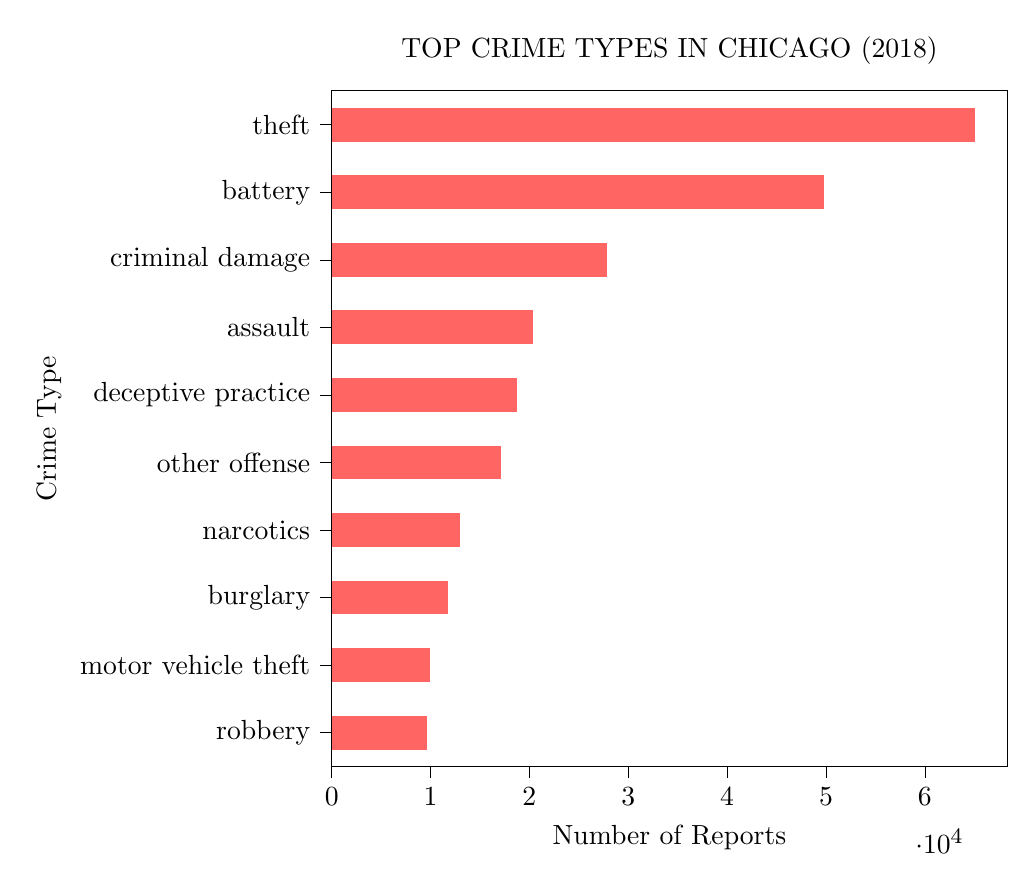
\begin{tikzpicture}

\definecolor{color0}{rgb}{1,0.4,0.388235294117647}

\begin{axis}[
height=4in,
tick align=outside,
tick pos=left,
title={\printsection{\MakeUppercase{Top Crime Types in Chicago (2018)}}},
width=4in,
x grid style={white!69.01960784313725!black},
xlabel={Number of Reports},
xmin=0, xmax=68332.95,
xtick style={color=black},
y grid style={white!69.01960784313725!black},
ylabel={Crime Type},
ymin=-0.5, ymax=9.5,
ytick style={color=black},
ytick={0,1,2,3,4,5,6,7,8,9},
yticklabels={robbery,motor vehicle theft,burglary,narcotics,other offense,deceptive practice,assault,criminal damage,battery,theft}
]
\draw[fill=color0,draw opacity=0] (axis cs:0,-0.25) rectangle (axis cs:9683,0.25);
\draw[fill=color0,draw opacity=0] (axis cs:0,0.75) rectangle (axis cs:9987,1.25);
\draw[fill=color0,draw opacity=0] (axis cs:0,1.75) rectangle (axis cs:11729,2.25);
\draw[fill=color0,draw opacity=0] (axis cs:0,2.75) rectangle (axis cs:12987,3.25);
\draw[fill=color0,draw opacity=0] (axis cs:0,3.75) rectangle (axis cs:17125,4.25);
\draw[fill=color0,draw opacity=0] (axis cs:0,4.75) rectangle (axis cs:18716,5.25);
\draw[fill=color0,draw opacity=0] (axis cs:0,5.75) rectangle (axis cs:20377,6.25);
\draw[fill=color0,draw opacity=0] (axis cs:0,6.75) rectangle (axis cs:27806,7.25);
\draw[fill=color0,draw opacity=0] (axis cs:0,7.75) rectangle (axis cs:49781,8.25);
\draw[fill=color0,draw opacity=0] (axis cs:0,8.75) rectangle (axis cs:65079,9.25);
\end{axis}

\end{tikzpicture}
\par}
\section{Data Augmentation \& APIs}
\subsection{Chicago Crime Reports, Augmented with ACS Demographic Information}
\section{Analysis \& Communication}
\subsection{Changes in Crime, 2017-2018}
\subsection{Analysis of Jacob Ringer's Claims}
\subsection{Key Findings}
\subsection{Caveats \& Limitations}
\section{Probability Exercise}
\begin{enumerate}[a)]
\item 
\item 
\item 
\end{enumerate}

\end{document} 
